\documentclass[10pt,conference,compsocconf]{IEEEtran}

\usepackage{hyperref}
\usepackage{graphicx}	% For figure environment
\usepackage{subcaption}


\begin{document}
\title{Machine Learning - Higgs Boson Project}

\author{
  Lucien Michaël Iseli, Florian Maxime Charles Ravasi and Jules Eliot Gottraux\\
  \textit{Master of Data Science, EPFL, Switzerland}
}

\maketitle

\section{Introduction}
In this project we try to determine if a given event's signature was the result of a Higgs boson (signal) or some other particle (background) thanks to a vector representing the decay signature of an event. The dataset is provided by the EPFL on the website AIcrowd and seperated into two parts: a test and a training set. Therefore, the goal is to choose an appropriate machine learning model, such as logistic regression, least squares or ridge regression and train it on the training set, in order to ultimately get the best results on the test set.
\section{Feature engineering}
When we first loaded the raw data and ran a simple model, wether it be linear regression or logistic regression, we got an accuracy of 66\% on training. In fact the data is unbalanced, two thirds of the data points are not Higgs boson and the remaining third are Higgs boson. So it was as good as always saying no. We needed to process the data to improve our results. \\\\
To do that we first used visualization tools, as we can gain a lot of insights on the data using visualization. Thus, we plotted the distribution of each feature. To have a better view of how the values are distributed we displayed them for each prediction, picking the same amout of $-1$ and $1$ predictions. Here is a typical example of which we learned a lot:
\begin{figure}[h!]
  \centering
  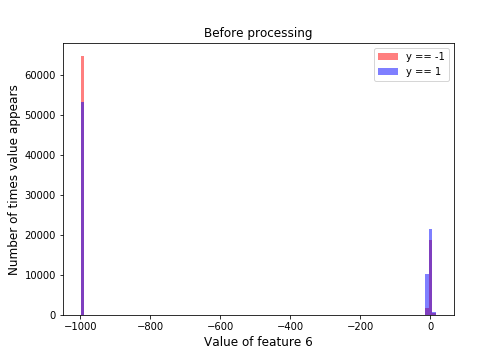
\includegraphics[width=\columnwidth]{graph-features/feature-06-raw.png}
  \caption{The feature 06 before processing}
	\label{fig:feature-06-raw}
\end{figure} \\
We noticed on figure \ref{fig:feature-06-raw} that the distribution is very strange and with this scale on the y-axis we can't really see exactly what's going on. But using this information and by going through the data there are features with many values set to exactly $-999$. Seems weird to have most of the values around 0 and a lot of them with exactly $-999$, we concluded that these values are in fact unknown.\\\\
Knowing that, we decided to normalize the data without taking into account the $-999$ values and then setting the $-999$ values to $0$. That way they shouldn't have much impact on the decision, since $0 \times w$ will give 0, thus not contribute. You can see the plot at figure \ref{fig:feature-06-processed}.
\begin{figure}[h!]
	\centering
  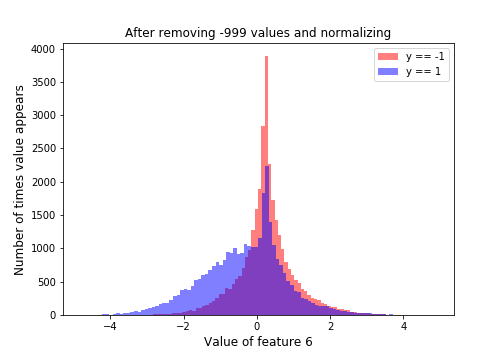
\includegraphics[width=\columnwidth]{graph-features/feature-06-processed.png}
  \caption{The feature 06 after processing, not displaying the $-999$ values}
	\label{fig:feature-06-processed}
\end{figure}

\section{Model choosing}

\section{Further improvements}

\begin{enumerate}
	\item{Copied 6 function we have to return from the labs}
	\item{Changed the functions we copied from the labs such that they always assume that vectors are represented in (N,1)}
	\item{Plotted distributions of features to gain insight}
	\item{Gradient descent on data to see what's going on}
	\item{Try to remove features based on the plots, the ones that look like they don't add anything}
	\item{Logistic regression, see if results make sense}
	\item{Try polynomial expansion to have better accuracy}
	\item{Try polynomial expansion with cross products to have better accuracy}
	\item{Realize that the weird distributions of many features with extreme variance are most likely due to the fact that -999 values are unknown values. Seems weird that many of the values are around zero, and many of them are exactly -999}
	\item{Normalize data without taking into account the -999 values, and set -999 values to 0. Such that they shouldn't affect the result as when 0 will be multiplied with the weight it'll be 0, i.e. not contribute.}
	\item{Replotted the distributions of the features after normalizing and removing the -999 values}
	\item{Notice that some plots look like uniform distribution or clearly don't give us insight on the result. => can remove them to have faster algorithm (NOT DONE YET)}
	\item{When plotting the distributions of features without unknown values we noticed someting very strange: all of the distributions are continuous except one! It only has 4 values}
	\item{We thought that maybe this value is some sort of category, thus maybe we should treat them differently => we trained them separatly, we separate them in 4 categories based on that feature and train them separatly}
	\item{Trained the model that way with linear regression (no expansion), obtained much better results}
	\item{Tried logistic regression but results weren't as good}
	\item{Tried to add feature expansion, square and sqrt (without cross products)}
\end{enumerate}

\end{document}
